\section{Methodology} \label{SettingtheStage}
We deemed two groups of research participants would be relevant to this survey- AI practitioners and lawmakers.  On one hand, practitioners often make the design decisions and have higher ethical responsibilities compared to others. Practitioners often make the design decisions of complex autonomous systems with less ethical knowledge. The magnitude of risks in AI systems makes practitioners responsible for understanding ethical attributes. To achieve reliable outcomes, it is essential to know the practitioners understanding of AI ethics principles and challenges. 

On the other hand, law resolves everyday conflicts and sustains order in social life. People consider law an information source as it impacts social norms and values \cite{AR11}. The aim of considering this type of population (lawmakers) is to understand the application of the law to AI ethics. The data collected from legislation personnel will uncover the question, of whether standing AI ethics principles are sufficient, or is there a need for innovative standards \cite{AR11}? 

We used industrial collaboration contacts to search the AI practitioners and sent a formal invitation to participate in this survey. Moreover, various law forums across the world were contacted and requested to participate in this study. The targeted populations were approached using social media networks including LinkedIn, WeChat, ResearchGate, Facebook, and personal email addresses. The overview of research methodology is depicted in Figure \ref{fig:Research Methodology}

\begin{figure}[t]
 \centering
  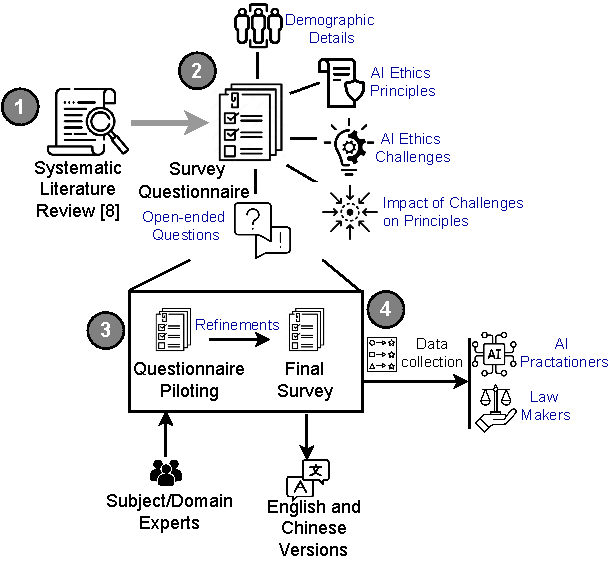
\includegraphics[width=0.48\textwidth]{Figures/AI-Ethics-Method.drawio.pdf}
 %\includegraphics[width=7cm,height=7cm]{Images/RQ1.drawio.pdf}
\caption{Overview of the research methodology}
\label{fig:Research Methodology}
\end{figure}

The survey instrument consisted of four core sections: 1) demographics 2) AI ethics principles 3) challenges 4) challenges impact on principles. The survey questionnaire also includes open-ended questions to know the novel principles and challenges that were not identified in the SLR study \cite{AR13}. The Likert scale is used to evaluate the significance of each principle and challenge and assess the severity level of the challenging factors. The survey instrument is structured both in English and Chinese language. The software industry in China is flourishing like never before, where AI is taking the front seat and is home to some of the leading technology giants in the world, such as Huawei, Alibaba, Baidu, Tencent, and Xiaomi. However, it would be challenging to collect the data from the Chinese industry because of the language barriers. Mandarin is the national and official language in China, unlike India, where English is commonly used for official purposes. Therefore, the Chinese version of the survey instrument is developed to cover the major portion of the targeted population. Both English and Chinese versions of the survey instrument are available online for replication \cite{replication}. 

The piloting of the questionnaire is performed by inviting three external subject/domain experts. The experts' suggestions were mainly related to the overall design, and understandability of the survey questions. The suggested changes were incorporated, and the survey instrument was finalized based on the authors' consensus (see Figure \ref{fig:Research Methodology}). The final survey instrument was online deployed using Google forms (English version) and Tencent questionnaire (Chinese version). The first two authors engaged with the data collection process, while the next co-authors frequently monitored/screened the participants' responses. The data collection process was started in September 2021 and ended up in April 2022 with initial 107 total responses. It should be noted, we provided the consensus details in the information sheet of the survey questionnaire \cite{replication} and only considered the agreed responses for further analysis. 

The manual review revealed that eight responses were incomplete and we only considered 99 responses for the final data analysis.The third author mainly extracted and analysed the survey data. The descriptive data were analyzed using the frequency analysis approach. The frequency-based tables and charts are created for the identified AI ethics principles and challenges (see Section \ref{sec:Results}). Frequency analysis is more suitable for analyzing a group of variables and for both numeric and ordinal types of data \cite{bland2015introduction}. The significance of identified AI ethics principles and challenges is evaluated based on the level of agreement between the two types of populations (AI practitioners, lawmakers) (see Section \ref{sec:Statistical inferences (RQ3)}). The same data analysis approach has been used in different other similar nature of studies \cite{akbar2022srcmimm}\cite{khan2017systematic}\cite{niazi2016toward}. Finally, various Zoom consent meetings were called and invited all the authors to overview the study results and provide feedback. The study replication package is provided in \cite{replication}.



